\section{Roboterbau}

In diesem Teil werden die einzelne Schritte beschrieben, um den Roboter zu bauen. Dabei wird sich an dem Konzept von \acrshort{pren1} orientiert. Falls von dem Konzept abgewichen wird, wird dies erwähnt und begründet. Die Arbeit aus \acrshort{pren1} kann im elektronischen Anhang gefunden werden.

Die folgenden Kapitel sind unterteilt nach den einzelnen Epics und User Stories, die im vorgehenden Kapitel \ref{projektplanung} aufgelistet wurden. Dabei werden die Tätigkeiten beschrieben, inklusive Testprotokolle und -beschriebe.

TODO: Risikoverweise (welches Risiko vermindert/behoben? Double checkwith table from prev chapter 
TODO: Testprotokolle
TODO: Lessons Learned
TODO: Komponentendiagramme mit Schnittstellen falls sinnvoll

TODO: 
Was vorkommen muss:
• Produktbeschreibung des Funktionsmusters (Hauptteil)
- Übersichtszeichnungen / Übersichtsmodell
- Beschreibung der Komponenten
- Ablaufdiagramme, Blockdiagramme
- Beschreibung der Funktionalität der einzelnen Blöcke und deren Beziehungen
- Schnittstellenbeschreibungen
- Softwaresubsysteme
- Wichtige Berechnungen (Resultate)
- Beschreibung von Versuchen und Tests mit Ergebnissen (Zusammenfassung)

\subsection{Produktbeschreibung}

In diesem Kapitel wird der Roboter als Gesamtsystem beschrieben. Dabei wird das Funktionsmuster mit einem Ablaufdiagramm beschrieben und die einzelnen physischen und elektronischen Komponenten werden in Zeichnungen aufgezeigt.


Die folgende Grafik \ref{fig:ablauf} zeigt das geplante Funktionsmuster auf. Dieses Ablaufdiagramm stammt aus \acrshort{pren1} und dient zur Erinnerung, genauere Informationen koennen aus der angehaengten PREN 1 Dokumentation entnommen werden.

\begin{figure}[H]
\centering
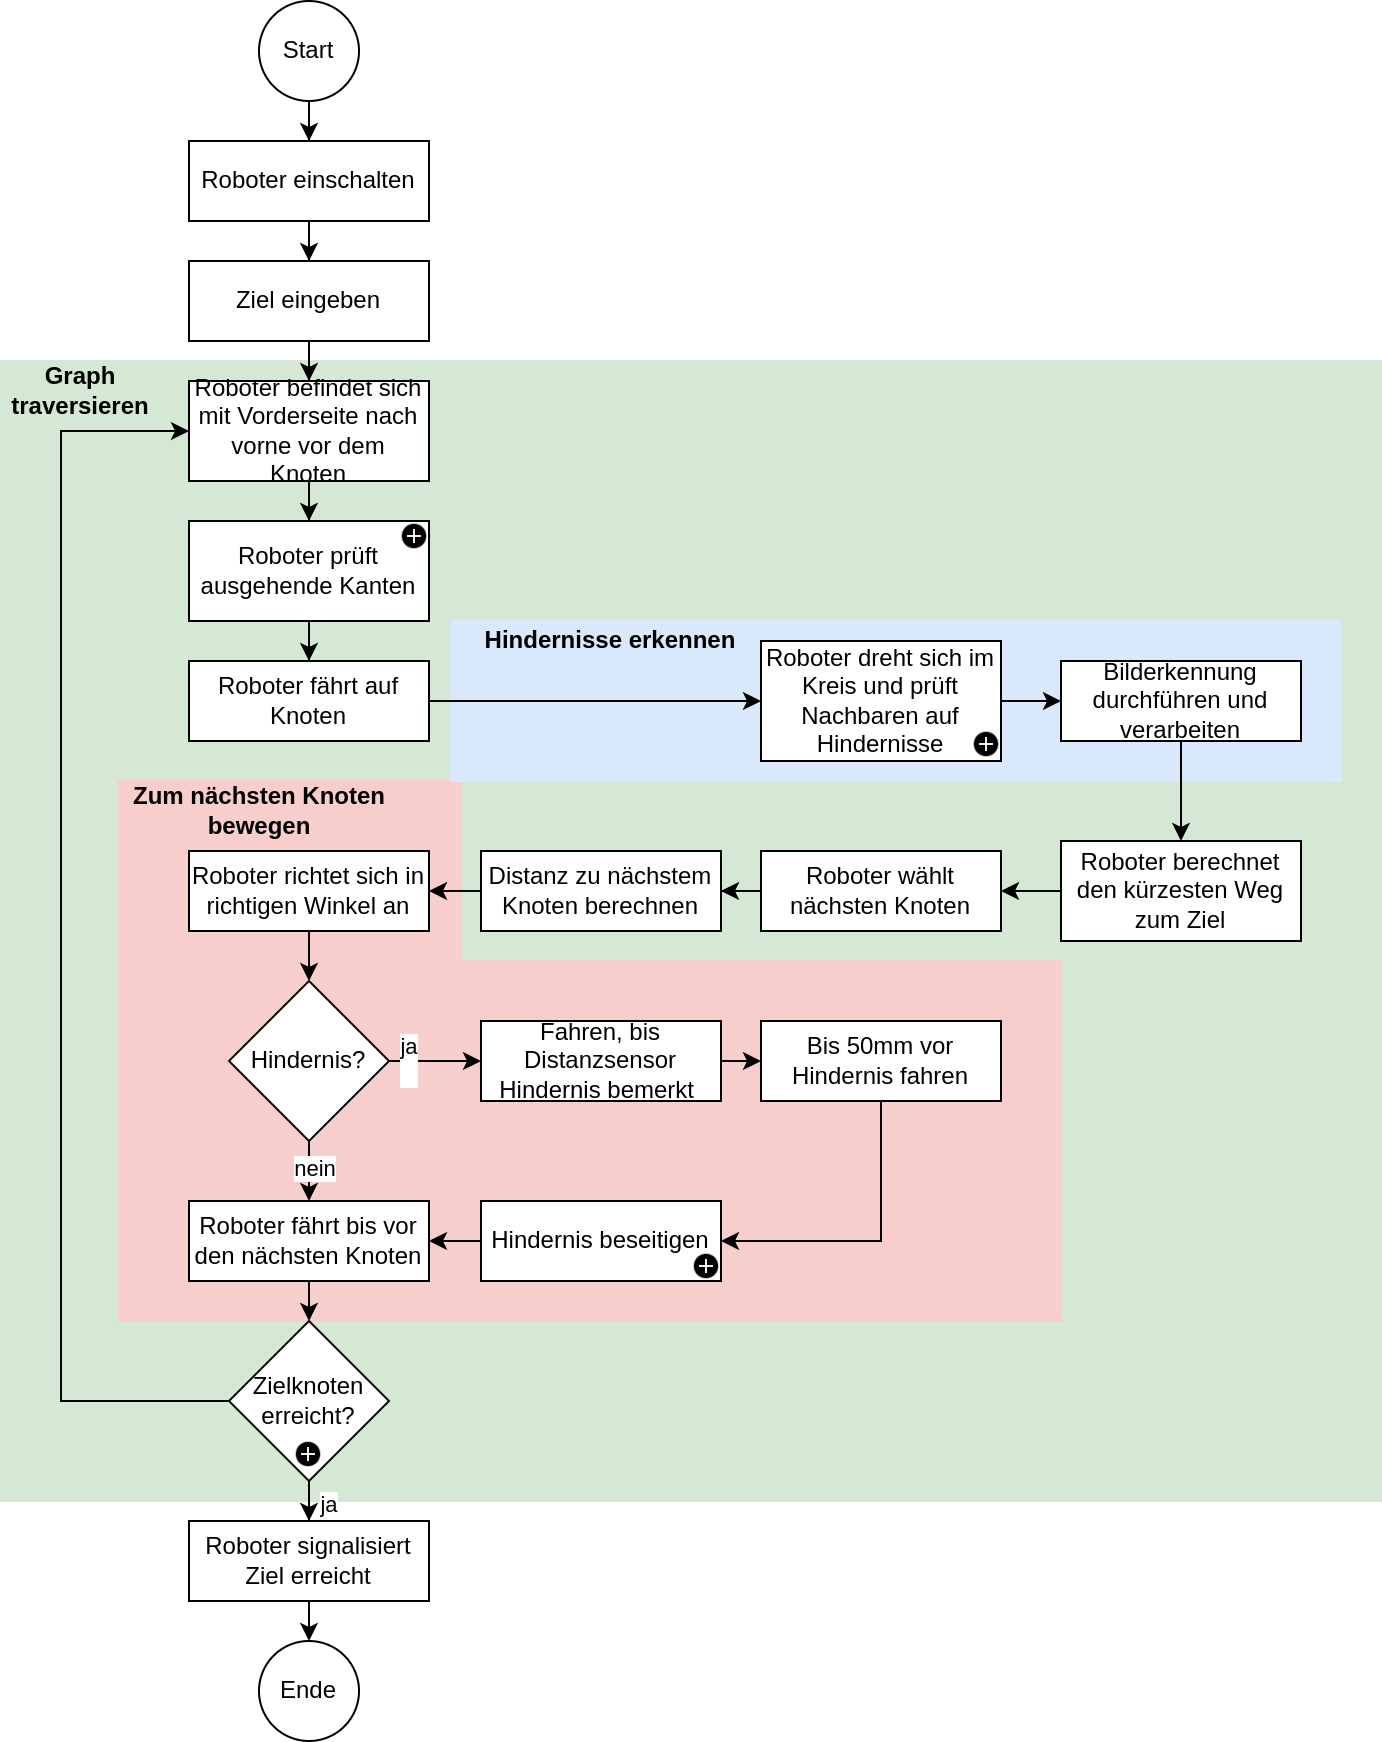
\includegraphics[width=\textwidth]{assets/gesamtkonzept/ablaufdiagramm.png}
\caption{Gesamtkonzept Ablaufdiagram}
\label{fig:ablauf}
\end{figure}

Damit dieses Funktionsmuster umgesetzt werden kann, wird ein Produkt mit folgenden Komponenten auf Grafik \ref{fig:components} gebaut. Die Grafik ist zeigt lediglich das Konzept mit den noetigen Komponenten und nicht das tatsaechliche Aussehen des Roboters.

\begin{figure}[H]
\centering
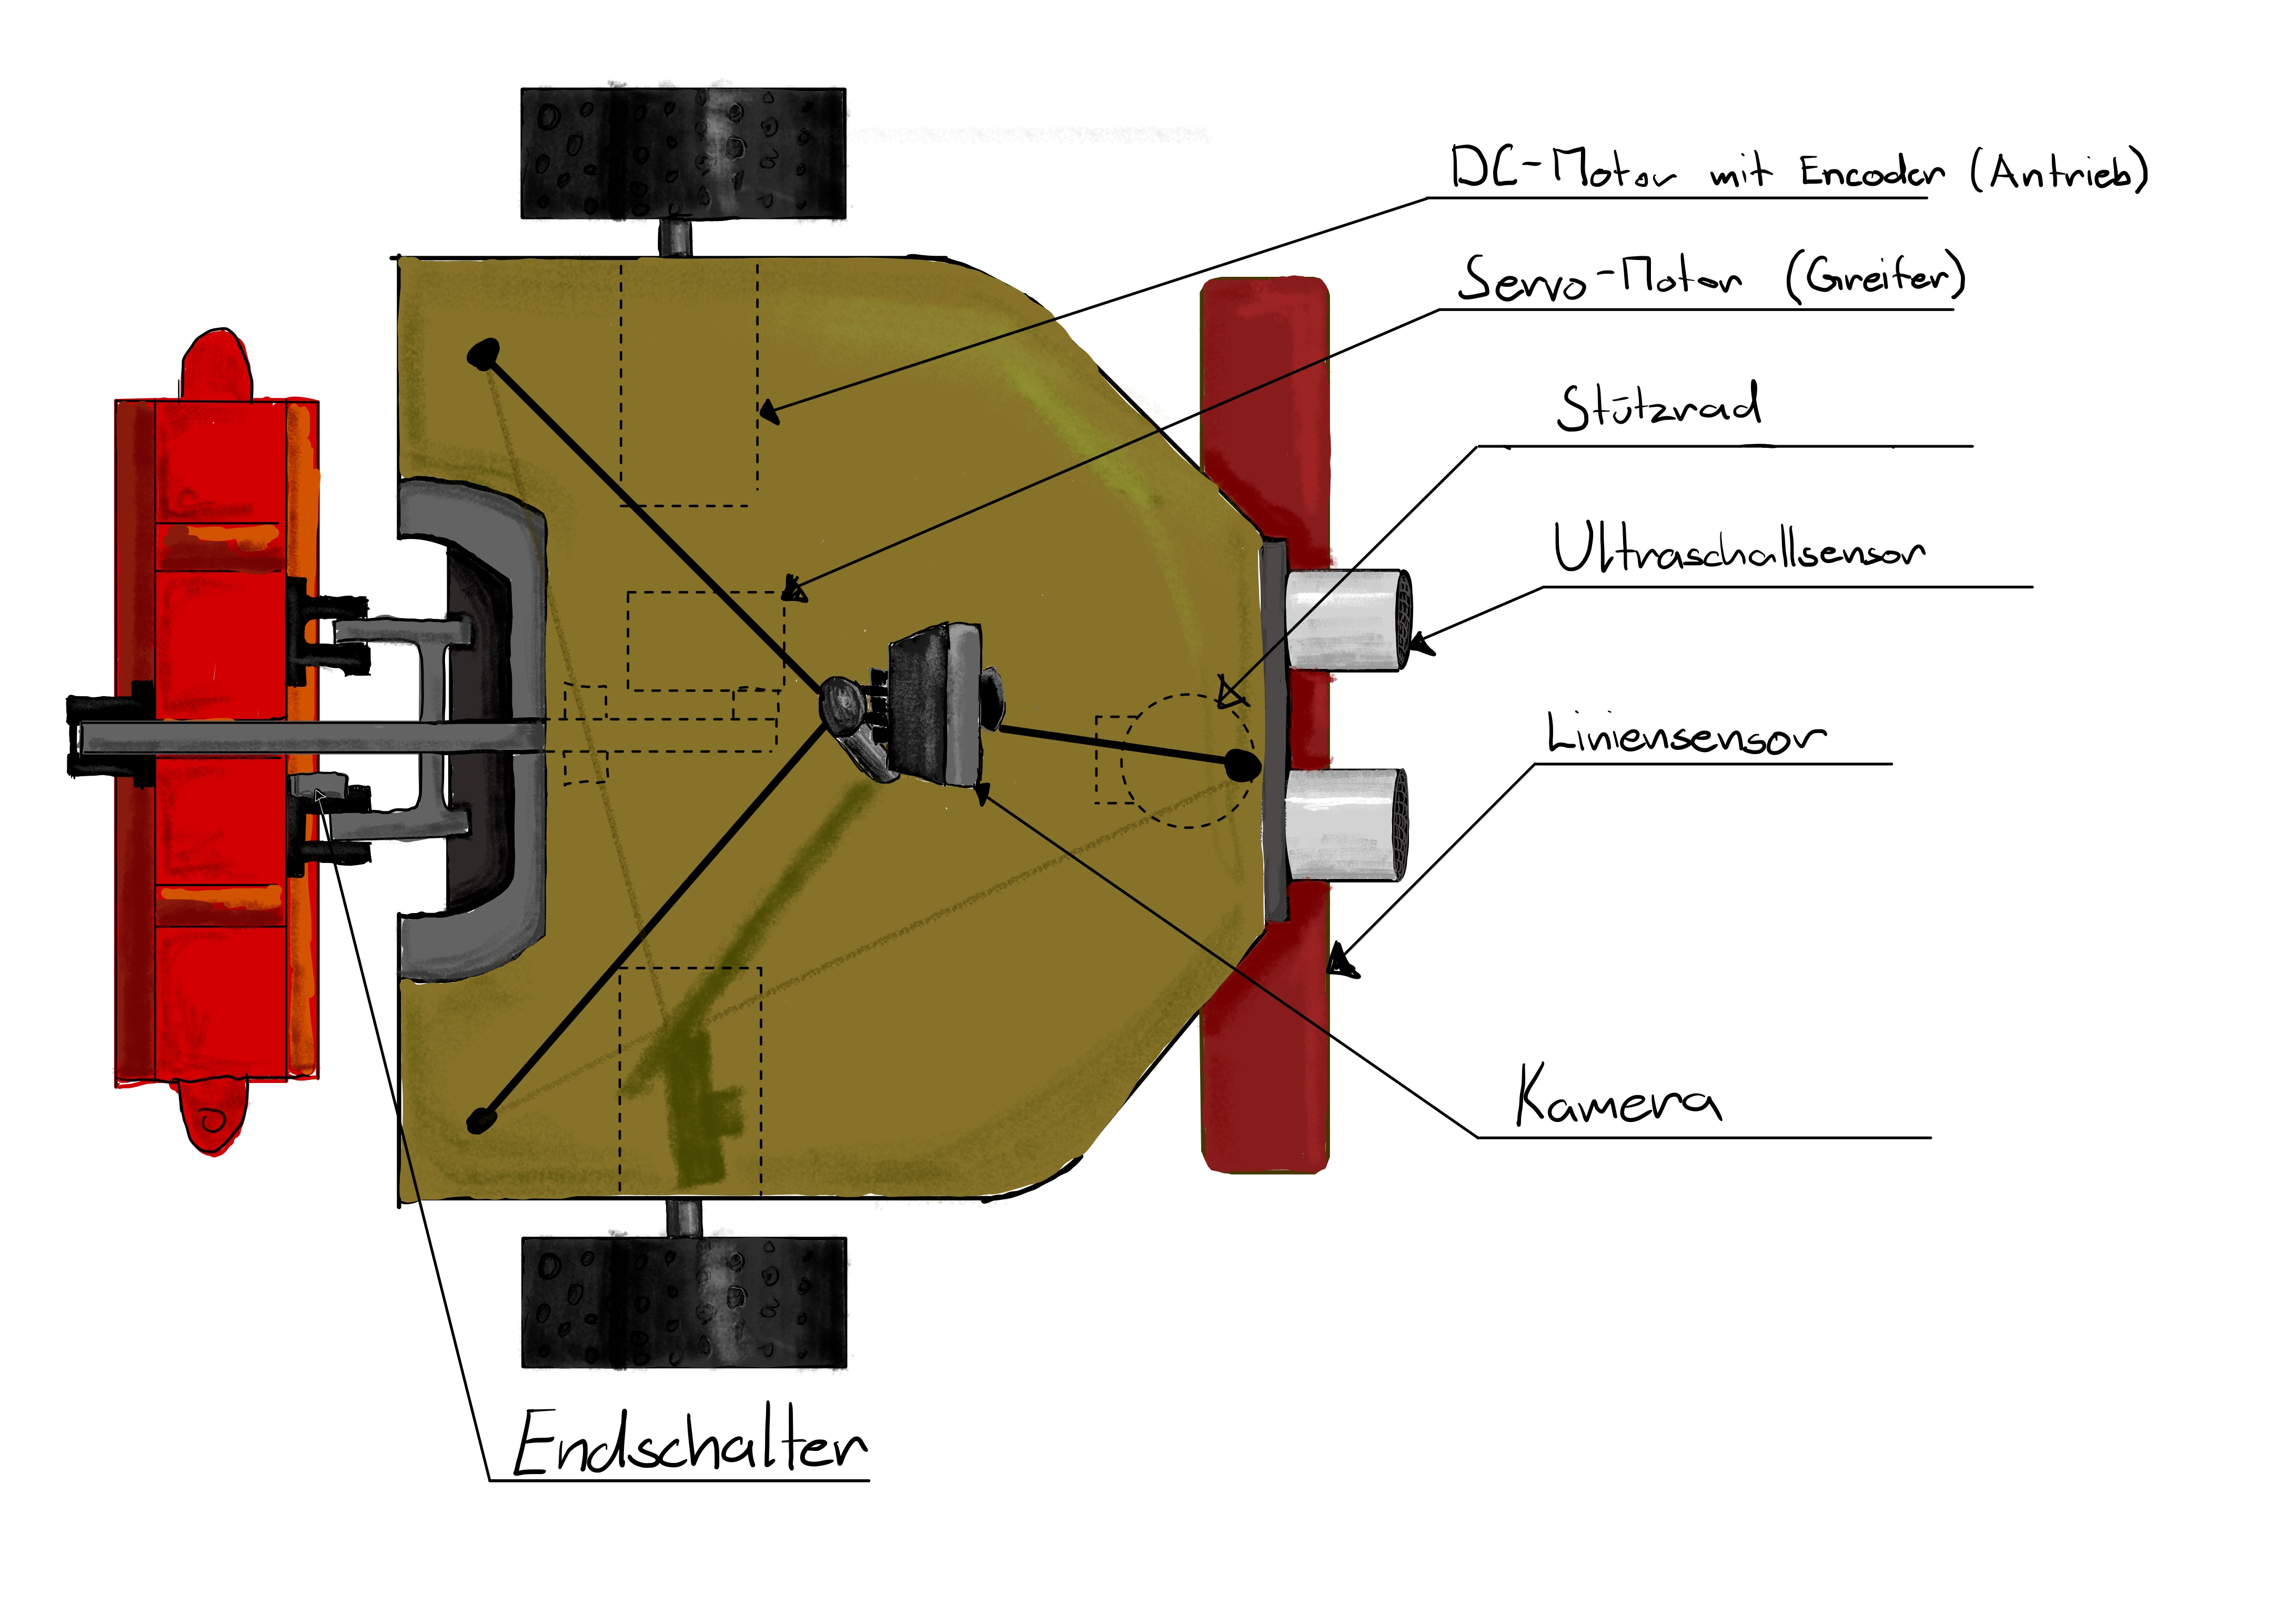
\includegraphics[width=\textwidth]{assets/gesamtkonzept/Skizze-Fahrzeugkonzept-Beschriftet.jpg}
\caption{Komponenten des Roboters}
\label{fig:components}
\end{figure}

Die einzelnen elektronischen Teile im Roboter bilden das Gesamtsystem ersichtlich auf Grafik \ref{fig:electro-components}. Dieses sorgt dafuer, dass sich der Roboter wie geplant autonom fortbewegen kann.

\begin{figure}[H]
\centering
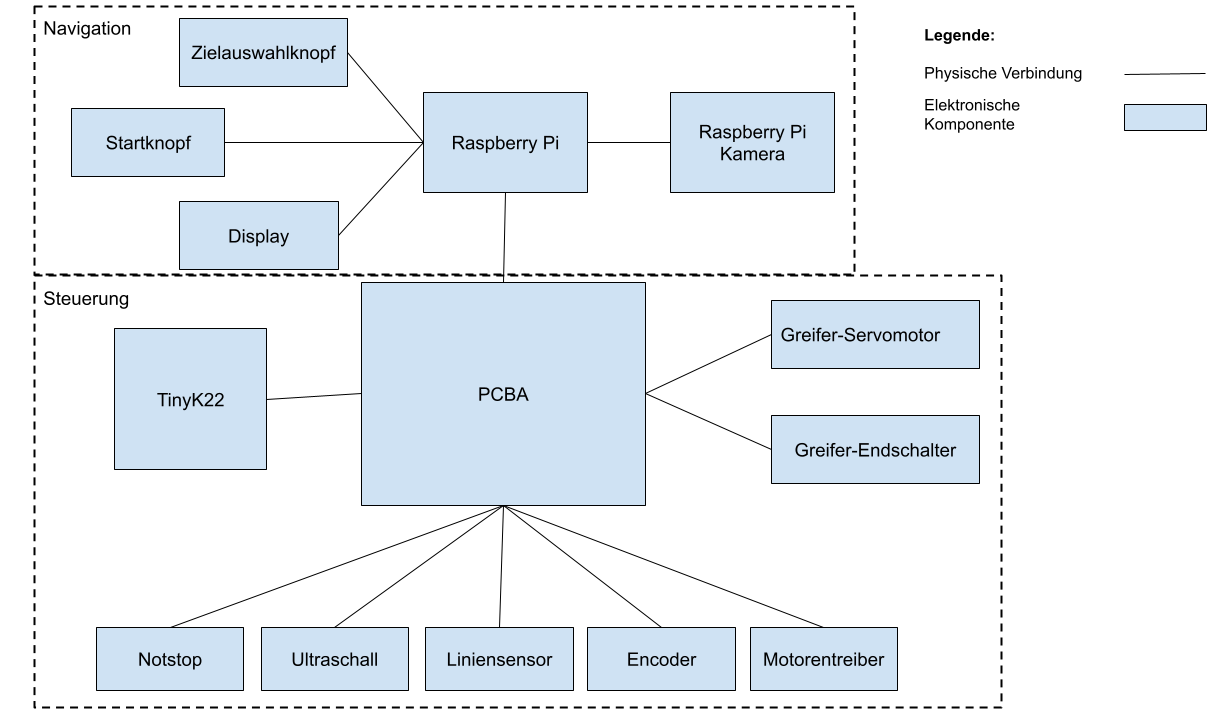
\includegraphics[width=\textwidth]{assets/gesamtkonzept/electronics.png}
\caption{Elektronische Komponenten des Roboters}
\label{fig:electro-components}
\end{figure} 

\newpage

%%%%%%%%%%%%%%%%%Epic 1%%%%%%%%%%%%%%%%%%%%%%%%%%%%%%%%%%%%%%%%%%%%%%%%%%%%%%%
\subsection{Fortbewegung mit geregelter Geschwindigkeit}

\subsubsection{Print Circuit Board Design}
\label{pcb}

Um eine zuverlässige Kontaktierung der einzelnen Komponenten sicherzustellen, wird im Rah-
men von Pren 2 ein Verbindungs-PCB \ref{fig: Verteiler PCB} entwickelt. Dieses PCB übernimmt das Management der
Spannungsversorgung für den Raspberry Pi und den TinyK22. Zudem werden sämtliche Signale,
die vom TinyK22 erfasst und verarbeitet werden sollen, entsprechend verbunden.

\begin{figure}[H]
\centering
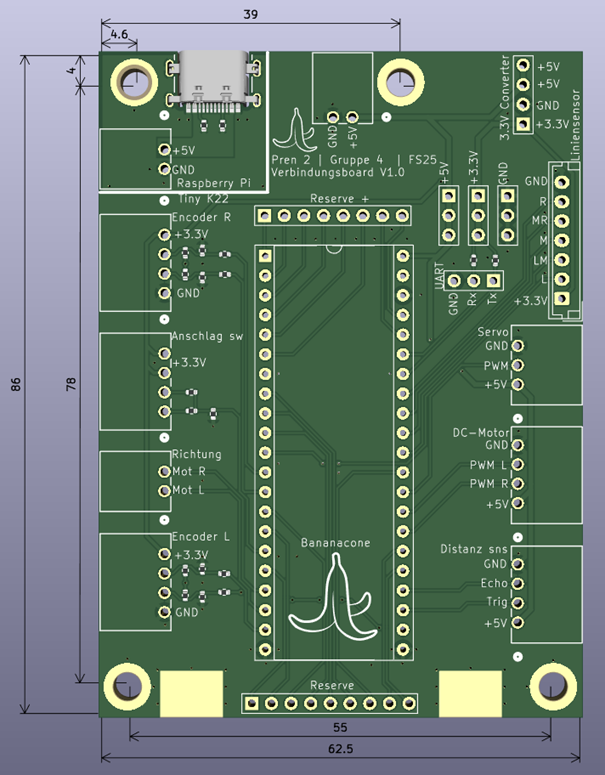
\includegraphics[width=5cm, height=6cm]{assets/ET/PCB/VerteilerPCB_unbestueckt.png}
\caption{Verteiler PCB}
\label{fig: Verteiler PCB}
\end{figure}

Von dem PCB wurden fünf Exemplare bestellt. Ebenso sind von dem TinyK22 mehrere Exemplare vorhanden \ref{fig: Verteiler PCBA}. Somit ist das Risiko der kaputten Elektroteile nicht mehr relevant.

\begin{figure}[H]
\centering
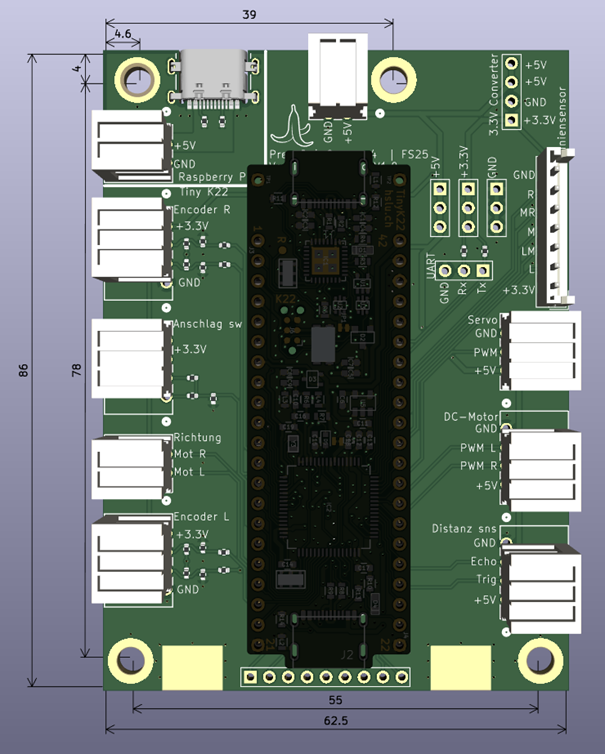
\includegraphics[width=5cm, height=6cm]{assets/ET/PCB/VerteilerPCB_bestueckt.png}
\caption{Verteiler PCBA}
\label{fig: Verteiler PCBA}
\end{figure}


\subsubsection{Motoren ansteueren und auslesen}

Nachdem die erste Ausführung der Software für die Motoren mit den beiden Encodern vorhanden war, wurde der implementierte Code mithilfe eines provisorischen Aufbaus getestet. Unter einem provisorischen Aufbau versteht man die Verwendung eines Breadboards mit dem TinyK22 und einem Speisegerät \ref{fig: Motorentest}. Allerdings wurde bereits der ausgewählte Motortreiber verwendet, der später auch im Endprodukt verbaut wird. Nach einigen Schwierigkeiten bei der Initialisierung des Quadratur-Encoder-Modus auf dem TinyK22 konnten die ersten Meter erfolgreich gefahren werden. Mit den ersten Erkenntnissen aus dem Test konnte die Software weiter angepasst werden, um immer präzisere Fahrmanöver auszuführen.

TODO Endgültige Situation mit Encodern


\begin{figure}[H]
\centering
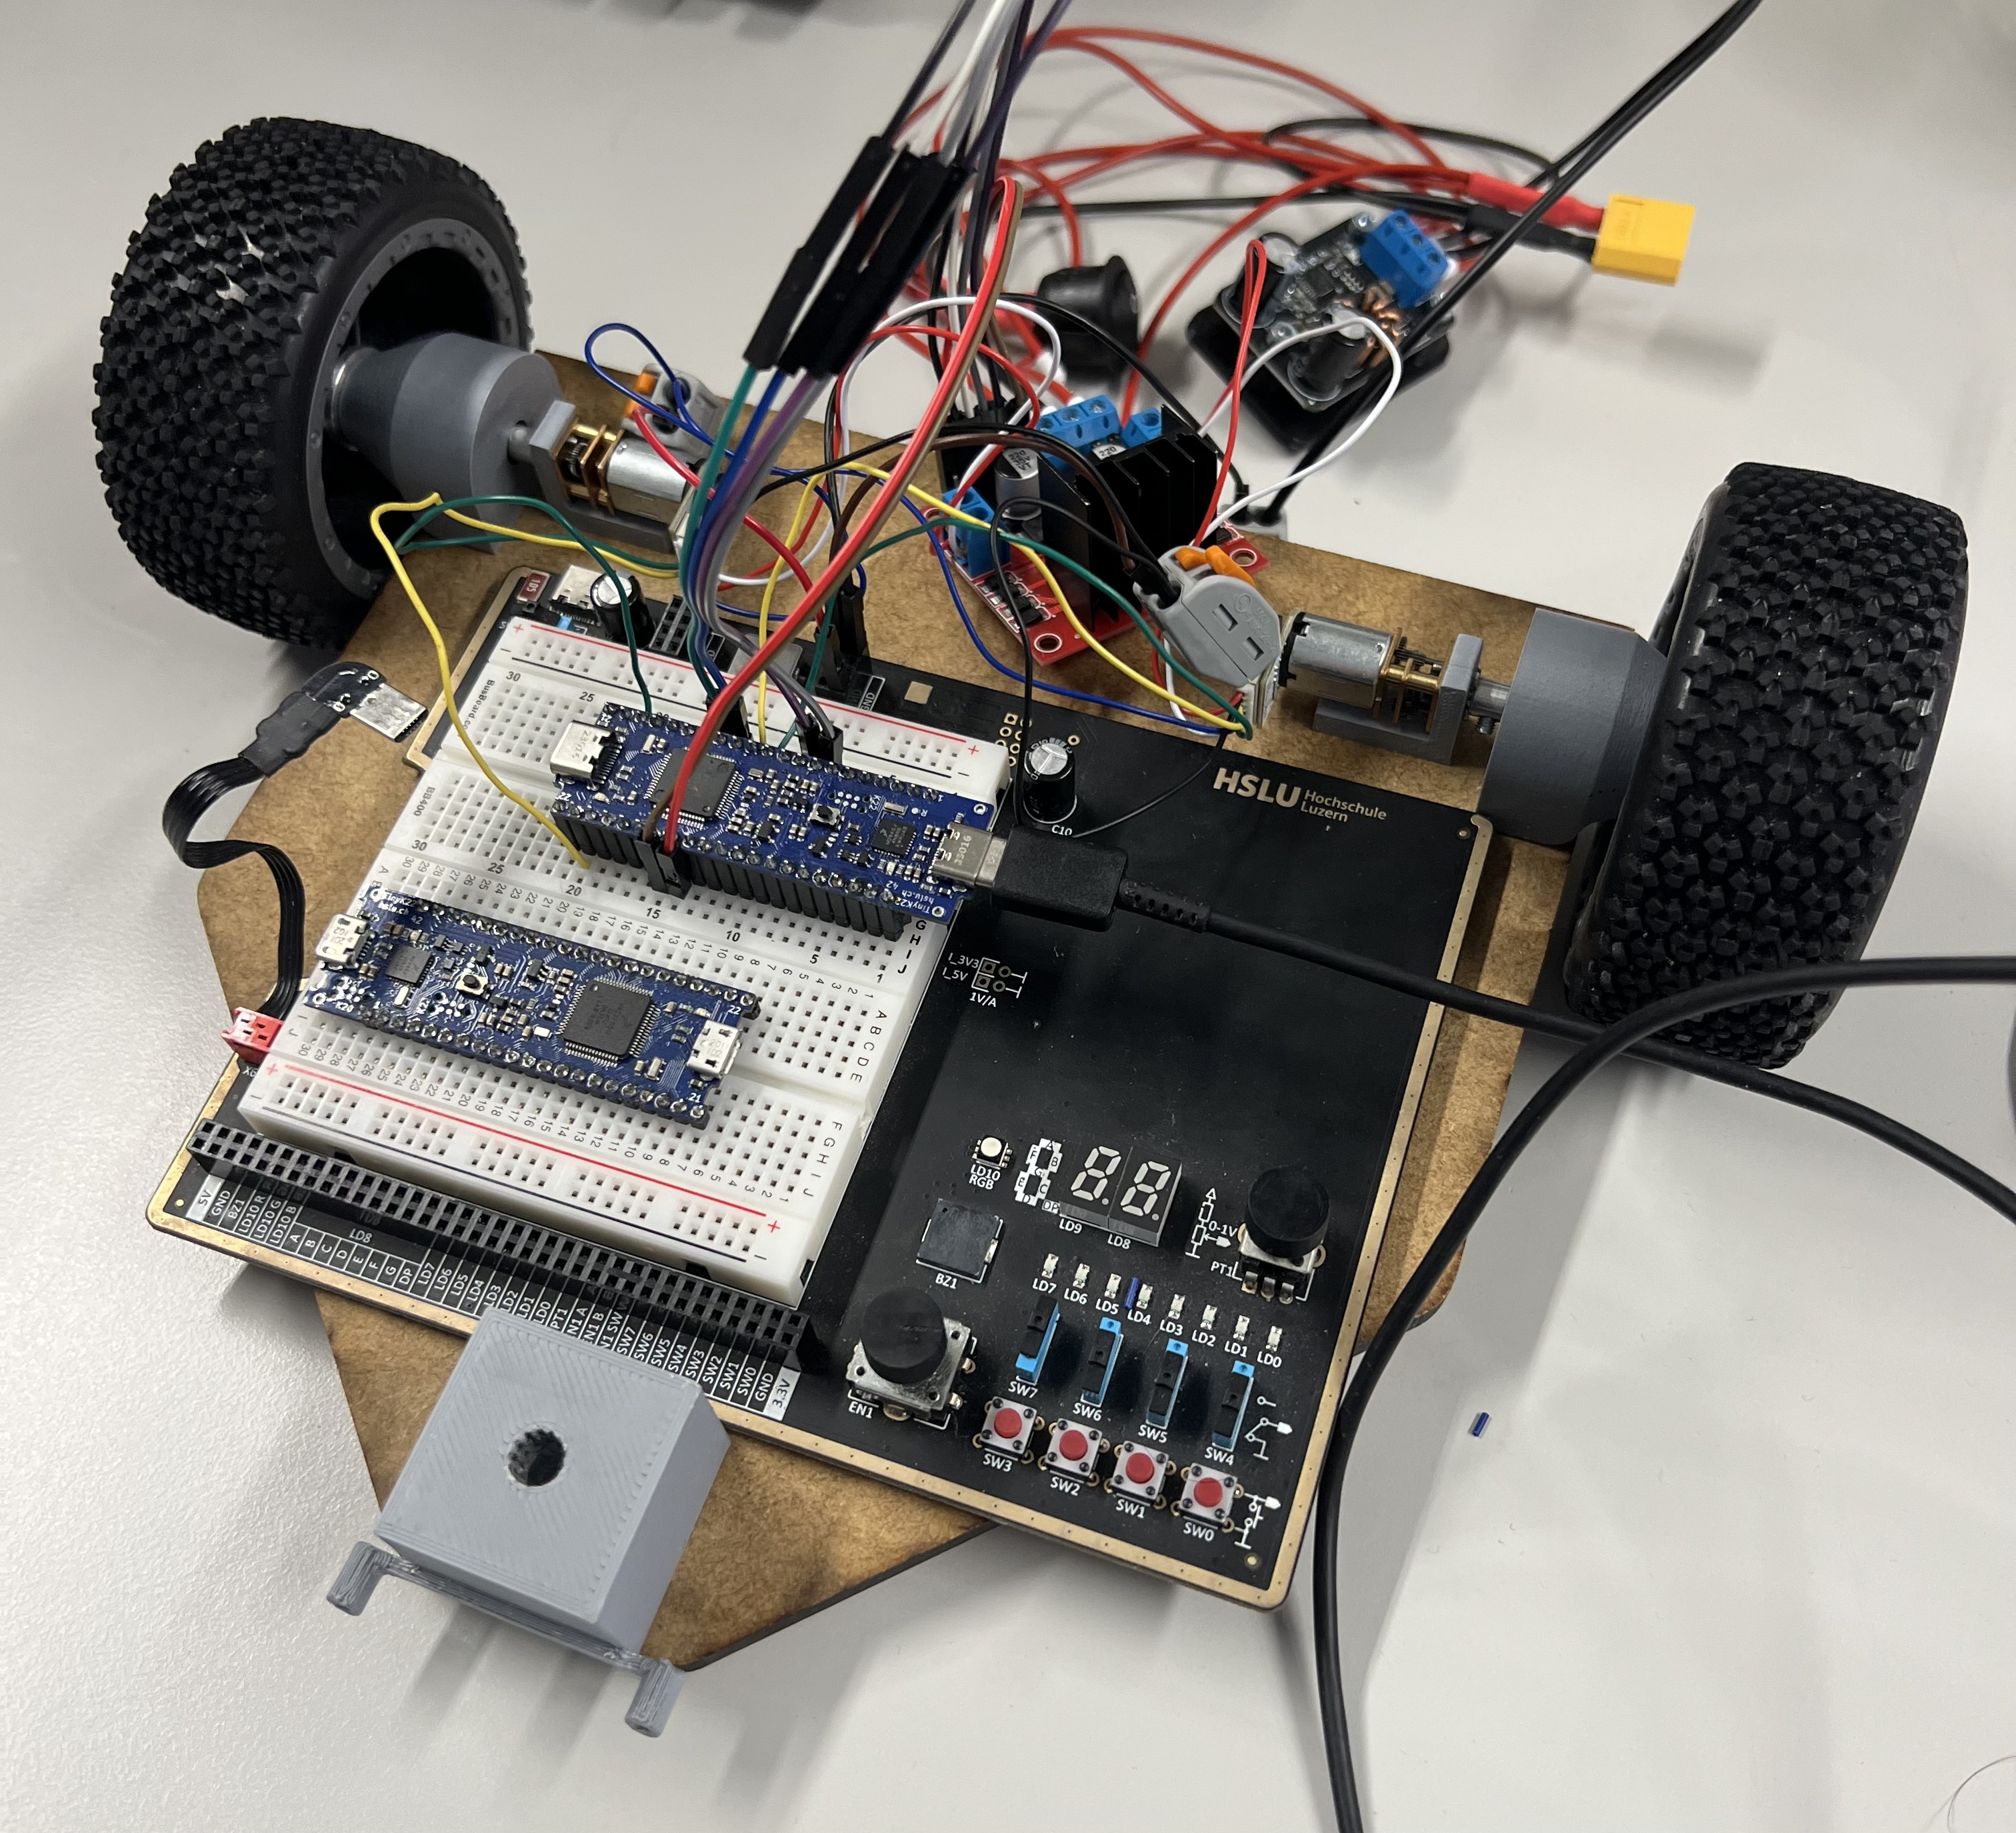
\includegraphics[width=10cm, height=8cm]{assets/ET/Motoren/Motorentest.jpeg}
\caption{Motorentest}
\label{fig: Motorentest}
\end{figure}

\subsubsection{Fahrwerk konstruieren}
\label{Fahrwerk konstruieren}

 Das Konzept für das Fahrwerk und die Grundplatte wurden analog zum Konzept aus PREN1 umgesetzt. Am Fahrwerk wurden gegenüber des Prototyps aus PREN1 einzig der Motorflansch und der Lenkrollenhalter angepasst. Beim Prototyp in PREN1 hat sich gezeigt, dass eine reine Presspassung für die Befestigung der Lenkrolle im Lenkrollenhalter aus PLA nicht ausreichend ist. Aus diesem Grund wird die Lenkrolle jetzt mithilfe eines M4 Gewindestifts geklemmt. Abb.\ref{fig: Lenkrollenhalter V2} 

\begin{figure}[H]
\centering
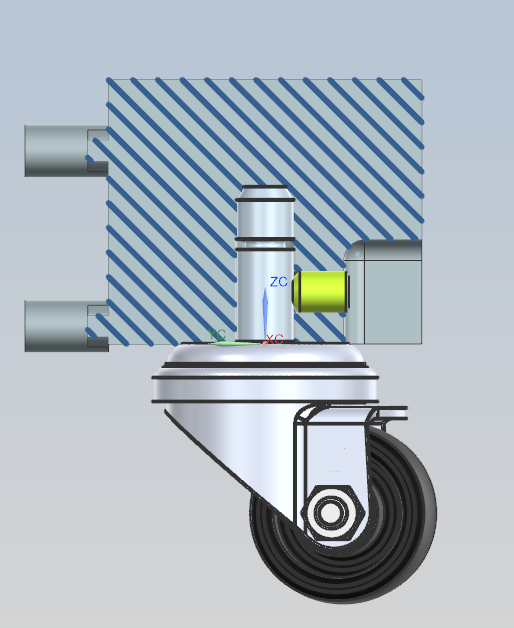
\includegraphics[width=5cm]{assets/MT/Lenkrollenhalter V2.png}
\caption{Lenkrollenhalter V2}
\label{fig: Lenkrollenhalter V2}
\end{figure}

Der Motorflansch wurde für den finalen Roboter leicht verstärkt. In  Abb. \ref{fig: Motorflansch V1/V2} sieht man in gelb die erste Version des Motorflansches wie er in PREN1 verbaut wurde. Blau eingefärbt die finale Version des Flansche mit einer Verstrebung. 

\begin{figure}[H]
\centering
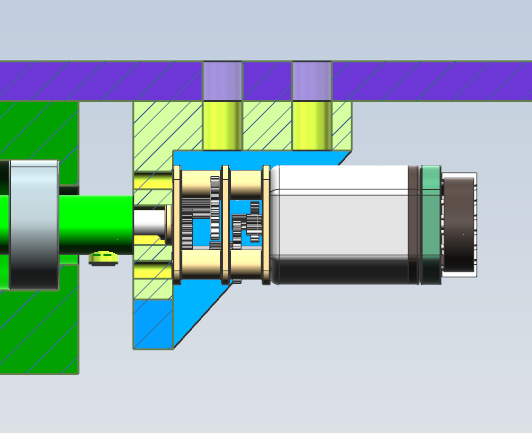
\includegraphics[width=5cm]{assets/MT/Motorflansch Vergleich.png}
\caption{Motorflansch V1/V2}
\label{fig: Motorflansch V1/V2}
\end{figure}

Die elektronischen Komponenten wie DC/DC-Konverter, Motortreiber oder RasberryPi werden nicht direkt auf die Grundplatte montiert, sondern auf Träger welche anschliessend auf die Grundplatte geschraubt werden. Die Träger wurden so konstruiert, dass die Kabel zwischen Träger und Bauteilen geführt werden können. (siehe Abb.\ref{fig: Träger für elektronische Komponenten}) Dieser Aufbau hatte in der frühen Testphase den Vorteil das alle elektronischen Komponenten provisorisch platziert werden konnten ohne einen Kurzschluss zu Riskieren. 

\begin{figure}[H]
\centering
\includegraphics[width=5cm]{assets/MT/Träger El Komponenten.jpg}
\caption{Träger für elektronische Komponenten werden zur Kabelführung verwendet}
\label{fig: Träger für elektronische Komponenten}
\end{figure}


\subsubsection{Greifer konstruieren}
\label{{Greifer konstruieren}

Der Klemm- und Hebemechanismus des Greifers sind Abhängig von der Federkraft und den Lagerstellen. Bei der Implementierung des Greifers musste darauf geachtet werden das die Lagerstellen nicht verschoben werden. In Abb \ref{fig:Greifer im Roboter} \& \ref{fig:Greifer Versuchsaufbau} sieht man, die für die Funktion wichtigsten Masse am Versuchsaufbau und am Fertigen Roboter. Die für für die Haltekraft verantwortliche Feder, sowie alle Haltebacken und Pendelstützen wurden vom Prototyp wiederverwendet. 

\begin{figure}[H]
  \centering
  \begin{minipage}[b]{0.45\textwidth}
    \centering
    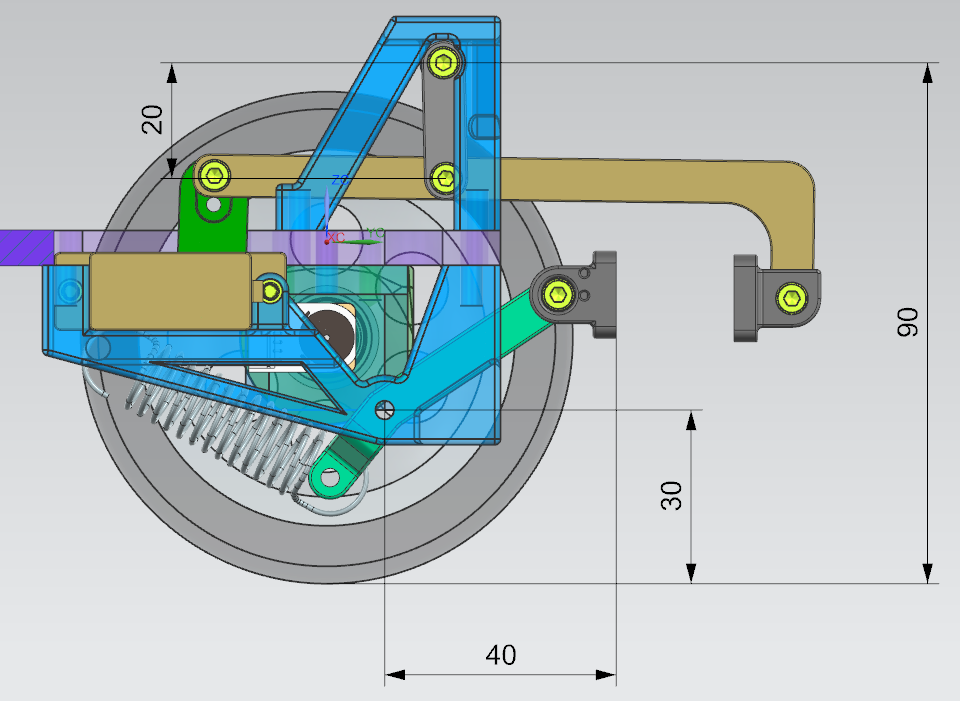
\includegraphics[height=5cm]{assets/MT/Greifer Montiert.png}
    \caption{Greifer im Roboter}
    \label{fig:Greifer im Roboter}
  \end{minipage}
  \hfill
  \begin{minipage}[b]{0.45\textwidth}
    \centering
    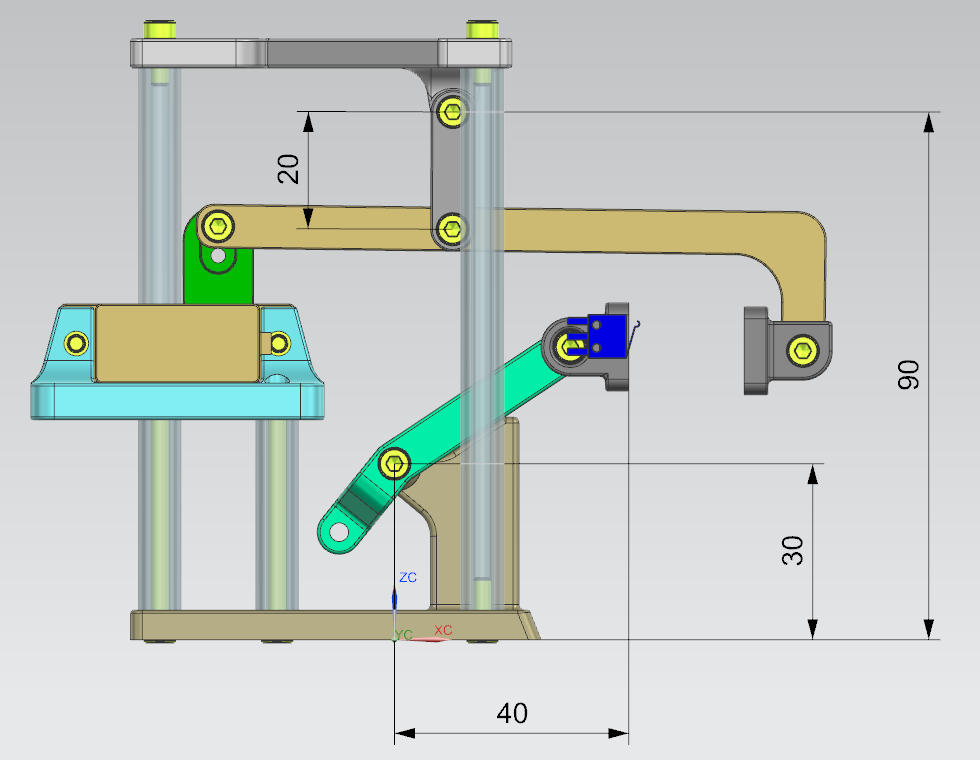
\includegraphics[height=5cm]{assets/MT/Greifer Prototyp.png}
    \caption{Greifer Versuchsaufbau}
    \label{fig:Greifer Versuchsaufbau}
  \end{minipage}
\end{figure}



-Raeder, PCB, Tiny, Akku, Motoren


\newpage
%%%%%%%%%%%%%%%%%Epic 2%%%%%%%%%%%%%%%%%%%%%%%%%%%%%%%%%%%%%%%%%%%%%%%%%%%%%%%

\subsection{Auf Linien des Graphes bewegen}

\subsubsection{Liniensensor auslesen}

In einem ersten Durchlauf wurde ein Code implementiert, um die Funktion mit dem TinyK22 zu testen. Mittels eines Timers wurden die einzelnen Pins in einem genügend grossen Zeitabstand von Vcc auf Input Capture umgeschaltet. Nach dem Umschalten auf Input Capture sollten sich die Kondensatoren je nach Reflexion des Untergrunds in unterschiedlichen Zeiten laden. Dieses Verhalten konnte im Testprogramm dann auch erfolgreich festgestellt werden, durch die unterschiedlichen Werte im Timer Register des Input Capture Modus.


TODO: schönes Bild vom Testgestell mit/für Liniensnesor

\subsubsection{Linie Folgen mit PD-Regelung}

Nachdem die Auslesung des Liniensensors erfolgreich getestet wurde, konnte die eigentliche Linienregelung implementiert werden. Abb. \ref{fig:Ausschnitt der Implementation der PD-Regelung}. Damit man möglichst dynamisch und ohne grosses schwingen fahren kann, wurd ein PD-Regler ausgewählt. Bei jedem Neustart des Roboters liest eine Kalibrierungsfunktion die Soll-Werte der einzelnen Sensoren ein. Beim Kalibrieren muss der Roboter immer in seiner Soll-Fahrposition stehen. Die periodisch aufgerufene Reglerfunktion berechnet dann aus dem Soll-Wert und dem aktuellen Sensorwert (Ist-Wert) die Abweichung. Diese Fehler werden zu einem Gesamtfehler mit einer Gewichtung der Sensoren von aussen nach innen zunehmend berechnet. Dieser Gesamtfehler wird dann mit dem P- und D-Anteil zu einem Korrekturwert weiter verrechnet. Der Proportionalanteil (P) sorgt dafür, dass das Fahrzeug bei einem grösseren Fehler stärker korrigiert, während der Differentialanteil (D) auf schnelle Änderungen des Fehlers reagiert und so Schwingungen dämpft. Der Korrekturwert wird dann genutzt um die beiden PWM Signale der Motoren zu senken oder erhöhen, je nach Abweichung zur Linie.

 \begin{figure}[H]
\centering
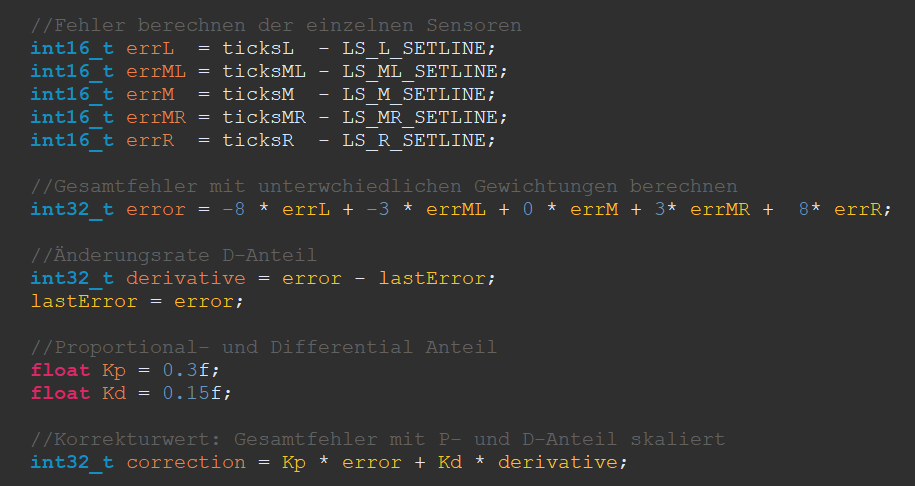
\includegraphics[width= \textwidth ]{assets/ET/PD-Regler/PD-Regler_Code_Pren2.png}
\caption{Ausschnitt der Implementation der PD-Regelung}
\label{fig:Ausschnitt der Implementation der PD-Regelung}
\end{figure}

 
\subsubsection{Abschirmung des Liniensensors}
Timo todo
\subsubsection{Liniensensor mit Abschirmung anbringen}

Nach dem ersten Test wurde der Liniensensor am Fahrzeug angebracht. Um Störeinflüsse von aussen zu vermeiden, wurde eine Abdeckung konstruiert, die jegliche Einstrahlung abschirmt. Dank diesem Aufbau konnte mit der weiteren Implementierung begonnen werden. Für die Feineinstellung wurden die einzelnen Sensorwerte auf dem Originalboden ausgemessen – ebenso auf dem Klebeband, da dies essenziell ist, um die Regelung sauber abzustimmen.



TODO: schönes Bild vom Schlussgestell mit Abschirmung des Liniensensors


\newpage
%%%%%%%%%%%%%%%%%Epic 3%%%%%%%%%%%%%%%%%%%%%%%%%%%%%%%%%%%%%%%%%%%%%%%%%%%%%%%

\subsection{Bis zum nächsten Knoten fahren}

\subsubsection{Kameranbindung}

...

\subsubsection{Distanz berechnen}

... POSSIBLY REMOVE TODO



... POSSIBLY REMOVE TODO

\subsubsection{Liniensensor}

Die Liniensensoren wurden wie geplant implementiert. Durch das Ummuxxen der Pins von GPIO-Output (High) auf den Input-Capture-Modus wird die Entladezeit eines Kondensators gemessen. Diese Zeit (ausgedrückt in Ticks) liefert Informationen darüber, ob sich das Fahrzeug über dem Soll-Fahrtweg befindet oder davon abweicht. Während der Fahrt werden die Sensor-Pins periodisch zwischen GPIO High und Input Capture umgeschaltet, um kontinuierlich neue Messwerte zu erhalten. Die erfassten Ticks werden in einer PD-Regelung weiter verarbeitet, welche die Abweichung zur Soll-Position (Linie) berechnet und entsprechend die Motoren nachsteuert. Diese Regelung ergänzt die Wegmessung über die Encodersensoren und erhöht die Spurtreue, indem sie sicherstellt, dass das Fahrzeug die Linie nicht verlässt.